% CS698I project report: Neighborhood Stability in Assignments on Graphs
% Build: pdflatex report.tex (twice)
\documentclass[11pt,a4paper]{article}
\usepackage[T1]{fontenc}
\usepackage{lmodern}
\usepackage[margin=2.5cm]{geometry}
\usepackage{amsmath,amssymb,amsthm}
\usepackage{booktabs}
\usepackage{enumitem}
\usepackage{tikz}
\usetikzlibrary{arrows.meta,positioning,calc,decorations.pathreplacing}
\usepackage{xcolor}
\usepackage[hidelinks]{hyperref}
\setlist{itemsep=2pt,topsep=4pt}
\setlength{\parskip}{4pt}

\newtheorem{theorem}{Theorem}
\newtheorem{proposition}{Proposition}
\newtheorem{lemma}{Lemma}
\newtheorem{claim}{Claim}
\newtheorem{observation}{Observation}
\theoremstyle{definition}
\newtheorem{definition}{Definition}
\newtheorem{example}{Example}
\theoremstyle{remark}
\newtheorem*{remark}{Remark}

\newcommand{\nlikes}{\nrightarrow}
\newcommand{\cP}{\mathcal{P}}

% ---------- figures (same style as the slides) ----------
\definecolor{ink}{HTML}{1F2933}
\definecolor{warn}{HTML}{C0392B}
\definecolor{good}{HTML}{1E8449}
\definecolor{muted}{HTML}{6B7280}
\definecolor{Afill}{HTML}{BFE3F8}\definecolor{Adraw}{HTML}{0072B2}
\definecolor{Bfill}{HTML}{FBE0A8}\definecolor{Bdraw}{HTML}{B87A00}
\definecolor{Cfill}{HTML}{B8E6D3}\definecolor{Cdraw}{HTML}{007A58}
\definecolor{Dfill}{HTML}{F2C9DF}\definecolor{Ddraw}{HTML}{A64D84}
\tikzset{
  ag/.style={circle,draw,thick,minimum size=7mm,inner sep=0pt,font=\bfseries},
  aga/.style={ag,fill=Afill,draw=Adraw}, agb/.style={ag,fill=Bfill,draw=Bdraw},
  agc/.style={ag,fill=Cfill,draw=Cdraw}, agd/.style={ag,fill=Dfill,draw=Ddraw},
  agg/.style={ag,fill=gray!12,draw=gray!60!black,font=\small},
  arc/.style={-{Stealth[length=2.4mm]},thick,draw=ink!85},
  like/.style={-{Stealth[length=2.4mm]},thick,draw=good},
  bad/.style={-{Stealth[length=2.4mm]},thick,draw=warn},
  sedge/.style={line width=1.3pt,draw=gray!55},
  hot/.style={line width=3.5pt,draw=warn!80},
  lab/.style={font=\scriptsize,text=muted},
}
\newcommand{\figtwopref}{%
  \node[aga] (a) at (0,1.6) {a}; \node[agc] (c) at (2.1,1.6) {c};
  \node[agb] (b) at (0,0) {b};   \node[agd] (d) at (2.1,0) {d};
  \draw[arc] (a) to[bend left=18] (c); \draw[arc] (c) to[bend left=18] (a);
  \draw[arc] (b) to[bend left=18] (d); \draw[arc] (d) to[bend left=18] (b);
  \draw[arc] (b) -- (a); \draw[arc] (d) -- (c);}
\newcommand{\figsixpref}{%
  \node[aga] (a) at (0,1.6) {a}; \node[agc] (c) at (2.1,1.6) {c};
  \node[agb] (b) at (0,0) {b};   \node[agd] (d) at (2.1,0) {d};
  \draw[arc] (c) -- (a); \draw[arc] (a) -- (b); \draw[arc] (a) -- (d);
  \draw[arc] (b) -- (d); \draw[arc] (d) -- (c);}
\newcommand{\pathseat}[4]{%
  \draw[sedge] (0,0) -- (4.5,0);
  \node[ag#1] (#1) at (0,0) {#1}; \node[ag#2] (#2) at (1.5,0) {#2};
  \node[ag#3] (#3) at (3,0) {#3}; \node[ag#4] (#4) at (4.5,0) {#4};}
\newcommand{\seatlabels}{\foreach \i in {1,...,4}{\node[lab] at ({(\i-1)*1.5},-0.6) {$v_{\i}$};}}
\newcommand{\sqseat}[6]{%
  \coordinate (#1) at (0,1.3); \coordinate (#2) at (1.3,1.3);
  \coordinate (#3) at (1.3,0); \coordinate (#4) at (0,0);
  \draw[sedge] (#1)--(#2)--(#3)--(#4)--cycle;
  \draw[hot] (#5)--(#6);
  \node[ag#1] (#1) at (#1) {#1}; \node[ag#2] (#2) at (#2) {#2};
  \node[ag#3] (#3) at (#3) {#3}; \node[ag#4] (#4) at (#4) {#4};}

\title{\textbf{Neighborhood Stability in Assignments on Graphs}\\[2mm]
\large A report on the paper by Aziz, Lisowski, Suzuki and Vollen (arXiv:2407.05240, 2024)}
\author{Ashik Stenny (230224) \qquad Achyuth H Warrier (230052)\\[1mm]
\small CS698I: Relational Structures in Games, IIT Kanpur \quad Instructor: Sunil Simon}
\date{14 November 2026}

\begin{document}
\maketitle

\begin{abstract}
We study the paper \emph{Neighborhood Stability in Assignments on Graphs} by Aziz, Lisowski, Suzuki and Vollen. Agents are placed on the vertices of a seat graph; each agent approves some other agents (binary preferences) and its utility is the number of approved neighbours. An assignment is \emph{neighbourhood stable} if no two \emph{adjacent} agents would both gain by swapping seats. The paper shows that such assignments need not exist (on balanced complete bipartite seat graphs), that swap dynamics can cycle even on a 4-cycle, but that a neighbourhood stable assignment always exists and can be computed in polynomial time on cycles and paths. On general seat graphs, one exists whenever the seat graph has enough leaves compared with the directed feedback vertex set number of the preference graph, and it can be computed in polynomial time when the preference graph is acyclic. We explain each result with a single running example, relate the paper to topics from the course (potential games, the finite improvement property, PLS, colouring games, hedonic games), and add our own observations: an exact characterisation of envy in the counterexample, a tighter $O(n^2)$ bound for the path algorithm, a five-agent instance showing why distance-2 stability fails on cycles, and two cases that the written proof of the main lemma for cycles does not cover, together with patches that we checked computationally.
\end{abstract}

\tableofcontents
\bigskip

\noindent\textbf{Notation for our contributions.} Statements that are ours and not in the paper are marked \textbf{[ours]}. Everything else follows the paper. Computational checks mentioned in the text are described in Appendix~\ref{app:verify}.

% =====================================================================
\section{Introduction and motivation}

\paragraph{The dinner party.} A host seats $n$ guests on $n$ fixed seats. Each guest likes some of the other guests (a yes/no opinion), and is happier the more liked guests sit next to them. If two guests sitting next to each other would \emph{both} be happier after exchanging seats, they will swap. Can the host choose a seating in which no two neighbours want to swap?

The paper opens with an equivalent organisational story: roles are designed in advance, members do not care which project they work on but do care which colleagues they work with, and the organisation wants to avoid pairs of members who would both prefer to swap roles. The model was introduced by Bodlaender et al.\ (2020) as \emph{hedonic seat arrangement} and has several recent follow-ups (Ceylan et al., Berriaud et al., Wilczynski).

\paragraph{Why a weaker stability notion.} As in hedonic games, where agents care only about who is in their coalition, stable outcomes in seating problems frequently fail to exist; Berriaud et al.\ found many non-existence results even when the seat graph is a path or a cycle. In the related Schelling games, Bil\`o et al.\ showed that allowing only \emph{local} swaps enlarges the set of equilibria, so that equilibria exist on more graph classes. The paper follows the same idea: it only forbids blocking pairs of \emph{adjacent} agents. This is natural for seating: to agree on a swap, two guests must talk, and at a table you talk to the people next to you, who are also exactly the people affecting your utility. It is also natural when agents only know the positions of their neighbours.

\paragraph{The question.} The paper asks: \emph{``For which classes of seat graphs is a neighborhood stable assignment guaranteed to exist under binary preferences?''}

\paragraph{Summary of results.}
\begin{center}\small
\renewcommand{\arraystretch}{1.25}
\begin{tabular}{@{}lll@{}}
\toprule
\textbf{Seat graph} & \textbf{Guarantee} & \textbf{Algorithm} \\
\midrule
$K_{t,t}$, $t\ge3$ odd & NS may not exist (Theorem~\ref{thm:kTT}) & -- \\
Cycle & NS always exists (Theorem~\ref{thm:cycle}) & $O(n^3)$ \\
Path & no blocking pair within distance 2 (Theorem~\ref{thm:path}) & $O(n^2)^{*}$ \\
Enough leaves ($\gamma\le\#$leaves) & NS exists (Theorem~\ref{thm:dfvs}) & poly.\ if $\cP$ is a DAG \\
\bottomrule
\end{tabular}
\end{center}
$^{*}$The paper states $O(n^3)$; $O(n^2)$ is our analysis of the same algorithm. Here NS abbreviates \emph{neighbourhood stable}, $\gamma$ is the directed feedback vertex set (DFVS) number of the preference graph, and DAG means directed acyclic graph.

% =====================================================================
\section{Model}

\begin{definition}[Instance]
A set $A=\{1,\dots,n\}$ of agents, an undirected \emph{seat graph} $G=(V,E)$ with $|V|=n$, and a directed \emph{preference graph} $\cP$ on $A$. We write $i\to j$ if $(i,j)$ is an arc of $\cP$ (agent $i$ \emph{approves}, or likes, agent $j$), and $i\nlikes j$ otherwise. An \emph{assignment} is a bijection $\pi:A\to V$.
\end{definition}

Write $N_\pi(i)$ for the agents seated next to $i$. The utility of agent $i$ is the number of approved neighbours,
\[ u_i(\pi)=\sum_{j\in N_\pi(i)}\mathbb{I}[i\to j]. \]

Let $\pi^{i\leftrightarrow j}$ denote $\pi$ with the seats of $i$ and $j$ exchanged. Agent $i$ \emph{envies} $j$ if $u_i(\pi^{i\leftrightarrow j})>u_i(\pi)$, and $i,j$ form a \emph{blocking pair} if each envies the other. An assignment is \emph{stable} if it has no blocking pair.

\begin{definition}[Neighbourhood stability]
An assignment $\pi$ is \emph{neighbourhood stable} (NS) if no blocking pair is assigned to adjacent vertices.
\end{definition}

\paragraph{Connection to hedonic games.} The paper notes that the problem is connected to hedonic games, in which agents are partitioned into coalitions according to their preferences over coalition members. \textbf{[Ours]} More precisely, utilities have the form of an additively separable hedonic game with $0/1$ values, except that an agent's ``coalition'' is its neighbourhood in the seat graph rather than a block of a partition.

\subsection{Running example}

We use the paper's Example 1 (Figure 2) throughout: four agents with $a\leftrightarrow c$, $b\leftrightarrow d$, $b\to a$ and $d\to c$, seated on a path of four seats.

\begin{figure}[h]
\centering
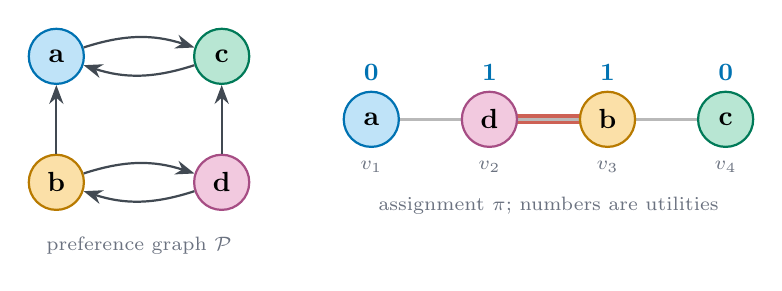
\begin{tikzpicture}
  \figtwopref
  \node[lab] at (1.05,-0.8) {preference graph $\cP$};
  \begin{scope}[xshift=4cm,yshift=0.8cm]
    \draw[hot] (1.5,0)--(3,0);
    \pathseat{a}{d}{b}{c}\seatlabels
    \foreach \x/\u in {0/0,1.5/1,3/1,4.5/0}{\node[font=\small\bfseries,text=Adraw] at (\x,0.6) {\u};}
    \node[lab] at (2.25,-1.1) {assignment $\pi$; numbers are utilities};
  \end{scope}
\end{tikzpicture}
\caption{The running example (paper's Fig.~2). Agents $b$ and $d$ form an adjacent blocking pair.}
\label{fig:running}
\end{figure}

Under $\pi=(a,d,b,c)$ we have $u_a=u_c=0$ and $u_b=u_d=1$. If $b$ and $d$ swap, giving $(a,b,d,c)$, then $d$ trades its neighbour $a$ (not approved) for $c$ (approved) and $b$ trades $c$ for $a$; both rise to $2$. So $b,d$ is an adjacent blocking pair and $\pi$ is not NS. The assignment $(a,b,d,c)$ is stable, hence also NS.

\subsection{How the notions relate}

Stable $\Rightarrow$ no blocking pair within distance $2$ (the notion studied by Berriaud et al.) $\Rightarrow$ NS. Deciding whether a stable assignment exists is computationally hard; the paper derives this from the exchange-stable roommates problem, which is NP-complete.

\begin{example}[NS is genuinely weaker; paper's Example 2, from Massand and Simon, IJCAI 2019]
Let the seat graph be two disjoint triangles and the preference graph a directed $6$-cycle $a\to b\to c\to d\to e\to f\to a$. No assignment is stable: in every assignment there are two agents at different triangles who both have utility $0$, and they block. Yet every assignment is NS, because adjacent agents share a triangle, and swapping two agents of a triangle leaves every neighbourhood unchanged. (We confirmed both facts over all $720$ assignments.)
\end{example}

\subsection{Why binary preferences}
Richer preferences fail almost immediately. With three non-negative values, there are four agents with no NS assignment on a cycle (the paper adapts the proof of Theorem~8 of Berriaud et al.). With values $\pm1$, the paper notes that ``it is easy to construct a counterexample of neighborhood stability on a path of length three'' by letting the friendship graph be a cycle. \textbf{[Ours]} One such instance: three agents on a path of three seats, each valuing its successor on a directed $3$-cycle at $+1$ and the other agent at $-1$; we checked that none of the six seatings is NS. Two non-negative values reduce to binary preferences without loss of generality.

% =====================================================================
\section{Neighbourhood stable assignments need not exist}

\begin{theorem}\label{thm:kTT}
For every $n=2t$ with $t\ge3$ odd, there is an instance with $n$ agents and no NS assignment.
\end{theorem}

\paragraph{Construction.} The seat graph is $K_{t,t}$ with sides $L$ and $R$. Agents form a top row $s_{11},\dots,s_{1t}$ and a bottom row $s_{21},\dots,s_{2t}$; indices are taken modulo $t$. Each agent approves exactly two agents: its \emph{twin} ($s_{1j}\leftrightarrow s_{2j}$) and its \emph{row successor} ($s_{ij}\to s_{i,j+1}$). So $\cP$ consists of $t$ directed 2-cycles and two directed $t$-cycles (Figure~\ref{fig:k33}).

\begin{figure}[h]
\centering
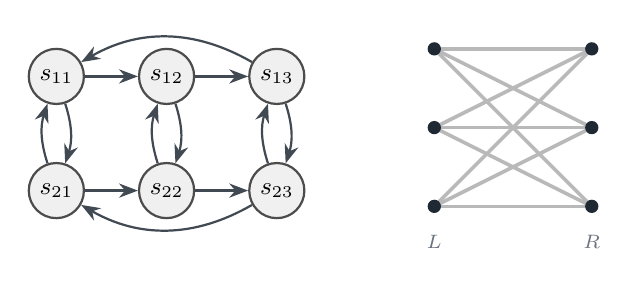
\begin{tikzpicture}[x=1.4cm,y=1.45cm]
  \foreach \j in {1,2,3}{
    \node[agg] (t\j) at (\j,1) {$s_{1\j}$};
    \node[agg] (b\j) at (\j,0) {$s_{2\j}$};
    \draw[arc] (t\j) to[bend left=18] (b\j); \draw[arc] (b\j) to[bend left=18] (t\j);}
  \draw[arc] (t1)--(t2); \draw[arc] (t2)--(t3); \draw[arc] (t3) to[bend right=30] (t1);
  \draw[arc] (b1)--(b2); \draw[arc] (b2)--(b3); \draw[arc] (b3) to[bend left=30] (b1);
  \begin{scope}[xshift=6.2cm,yshift=-0.2cm,x=1cm,y=1cm]
    \foreach \y in {0,1,2}{\foreach \z in {0,1,2}{\draw[sedge] (0,\y)--(2,\z);}}
    \foreach \y in {0,1,2}{\fill[ink] (0,\y) circle (2.4pt); \fill[ink] (2,\y) circle (2.4pt);}
    \node[lab] at (0,-0.45) {$L$}; \node[lab] at (2,-0.45) {$R$};
  \end{scope}
\end{tikzpicture}
\caption{Theorem~\ref{thm:kTT} for $t=3$ (paper's Fig.~1): preference graph (left) and seat graph $K_{3,3}$ (right).}
\label{fig:k33}
\end{figure}

\paragraph{Key simplification.} In $K_{t,t}$ the neighbours of an agent are exactly the agents on the other side, so an assignment is determined (for utilities) by the split into sides $L$ and $R$. Each agent approves exactly two agents, so its utility is the number of its two favourites on the other side. If $i$ swaps with $j$ on the other side, $i$'s new neighbours are its former side-mates together with $j$. The paper uses two sufficient conditions for $i$ to envy an agent $j$ on the other side:
\begin{itemize}
  \item[(C1)] both of $i$'s favourites are on $i$'s own side ($u_i=0$); then $i$ envies \emph{every} agent on the other side ($0\to2$);
  \item[(C2)] exactly one favourite is on $i$'s own side and $i\to j$; then $i$ envies $j$ ($1\to2$).
\end{itemize}

\begin{lemma}[\textbf{ours}]
In this instance, $i$ envies $j$ if and only if (C1) or (C2) holds.
\end{lemma}
\begin{proof}
If $i,j$ are on the same side, swapping changes nothing for $i$. Otherwise let $k$ be the number of $i$'s favourites on its own side. Then $u_i(\pi)=2-k$ and $u_i(\pi^{i\leftrightarrow j})=k+\mathbb{I}[i\to j]$. For $k=2$ this is $2>0$ (C1); for $k=1$ it is $1+\mathbb{I}[i\to j]>1$ iff $i\to j$ (C2); for $k=0$ the agent already has the maximum utility $2$.
\end{proof}

A blocking pair needs envy in both directions, and each direction may use either condition. Since agents on opposite sides are adjacent, any blocking pair across the sides violates NS. The proof considers two cases.

\paragraph{Case 1: some twin pair sits on one side.}
\begin{enumerate}
  \item A split twin pair contributes one agent to each side. Since both sides have $t$ agents, the together pairs must be shared equally: \emph{$L$ and $R$ contain the same number of together pairs}. Hence the number of agents in together pairs is even, and as $t$ is odd, at least one twin pair is split.
  \item Going around the indices, some together pair at index $j$ is followed by a split pair at $j+1$. Relabel so that $s_{1j},s_{2j},s_{1,j+1}\in L$ and $s_{2,j+1}\in R$.
  \item Both favourites of $s_{1j}$ are in $L$, so by (C1) it envies everyone in $R$.
  \item If some agent of $R$ had utility $0$, it would envy $s_{1j}$ by (C1) and they would block. So every agent of $R$ approves someone in $L$. For a together pair in $R$ at index $l$, the agent $s_{1l}$ approves $s_{2l}\in R$, so $s_{1,l+1}$ must be in $L$; likewise $s_{2,l+1}\in L$. Thus every together pair in $R$ at $l$ is followed by a together pair in $L$ at $l+1$.
  \item This map from together pairs in $R$ to together pairs in $L$ is injective, and both sets have the same size, so it is a bijection. In particular the pair at $j-1$ is together in $R$.
  \item Then $s_{1,j-1}\in R$ approves $s_{2,j-1}$ (own side) and $s_{1j}$ (other side), so it envies $s_{1j}$ by (C2). Together with step 3, $s_{1,j-1}$ and $s_{1j}$ block.
\end{enumerate}

\paragraph{Case 2: every twin pair is split.} Side $L$ contains one agent of every twin pair, so at least $\lceil t/2\rceil$ of its agents come from the same row, say the top row. These agents lie on the directed $t$-cycle $s_{11}\to\dots\to s_{1t}\to s_{11}$, whose largest independent set has size $\lfloor t/2\rfloor<\lceil t/2\rceil$ because $t$ is odd. Hence two consecutive top agents, say $s_{11},s_{12}$, are in $L$, and their twins $s_{21},s_{22}$ are in $R$. Now $s_{11}$ approves $s_{12}$ (own side) and $s_{21}$ (other side), and $s_{21}$ approves $s_{22}$ (own side) and $s_{11}$ (other side). By (C2) they envy each other.

\paragraph{The case $t=3$ in detail [ours].} Up to exchanging the sides there are $10$ splits. If some twins are together, each side has at most one together pair (two would need four agents), so Case 1 means \emph{one together pair on each side and one split pair}; there are $6$ such splits. For example, take $L=\{s_{11},s_{21},s_{12}\}$ and $R=\{s_{22},s_{13},s_{23}\}$. Twins $1$ are together and twins $2$ are split, so $j=1$; $s_{11}$ has utility $0$. The only remaining index is $3=j-1$, whose twins are together in $R$, and $s_{13}$ has utility $1$. Swapping $s_{11}$ and $s_{13}$ raises their utilities from $0$ to $2$ and from $1$ to $2$. The remaining $4$ splits are Case 2; for instance $L=\{s_{11},s_{12},s_{23}\}$, $R=\{s_{21},s_{22},s_{13}\}$, where $s_{11}$ and $s_{21}$ both go from $1$ to $2$ by swapping. In a triangle every two vertices are consecutive, which is why Case 2 is immediate for $t=3$. We confirmed by brute force that none of the $720$ assignments is NS.

\paragraph{Where oddness is used.} Case 1 needs a split twin pair, and Case 2 needs an odd cycle. \textbf{[Ours]} For even $t$ the construction does not work: for $t=4$, putting $s_{11},s_{13},s_{22},s_{24}$ on $L$ places every agent's twin and successor on the other side, so every agent has the maximum utility $2$ and the assignment is stable.

% =====================================================================
\section{Swap dynamics can cycle}

\emph{Swap dynamics} starts from an arbitrary assignment and lets adjacent blocking pairs swap until none remains.

\begin{proposition}\label{prop:loop}
There is an instance and an assignment from which swap dynamics never converge, even when the seat graph is a cycle of length $4$.
\end{proposition}

The instance (paper's Fig.~6) has $c\to a$, $a\to b$, $a\to d$, $b\to d$, $d\to c$. Figure~\ref{fig:loop} shows the four swaps. In each assignment the highlighted pair is the \emph{unique} adjacent blocking pair, so there is no choice of swap at any step.

\begin{figure}[h]
\centering
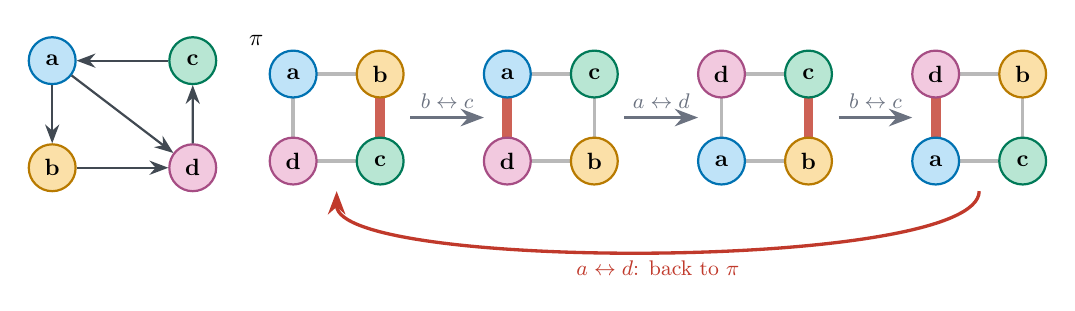
\begin{tikzpicture}[scale=0.85,every node/.style={transform shape}]
  \begin{scope}[xshift=-3.6cm,yshift=-0.1cm]\figsixpref\end{scope}
  \begin{scope}[xshift=0cm]\sqseat{a}{b}{c}{d}{b}{c}\node[font=\bfseries] at (-0.55,1.8) {$\pi$};\end{scope}
  \begin{scope}[xshift=3.2cm]\sqseat{a}{c}{b}{d}{a}{d}\end{scope}
  \begin{scope}[xshift=6.4cm]\sqseat{d}{c}{b}{a}{c}{b}\end{scope}
  \begin{scope}[xshift=9.6cm]\sqseat{d}{b}{c}{a}{d}{a}\end{scope}
  \foreach \x/\l in {1.75/{b\leftrightarrow c},4.95/{a\leftrightarrow d},8.15/{b\leftrightarrow c}}{
    \draw[-{Stealth},very thick,muted] (\x,0.65)--(\x+1.1,0.65) node[midway,above,font=\small] {$\l$};}
  \draw[-{Stealth},very thick,warn] (10.25,-0.45) to[out=-90,in=-90,looseness=0.32] node[below,font=\small] {$a\leftrightarrow d$: back to $\pi$} (0.65,-0.45);
\end{tikzpicture}
\caption{Proposition~\ref{prop:loop}. Left: preferences. Right: the cycle of swaps on a 4-cycle seat graph; red marks the unique blocking pair. Gains: $b,c$ go $0\to1$; $a$ goes $1\to2$ and $d$ goes $0\to1$.}
\label{fig:loop}
\end{figure}

\paragraph{Consequences and course connections.}
\begin{itemize}
  \item The four swaps form an \emph{improvement cycle}. In a finite game, the finite improvement property (FIP) is equivalent to having a generalised ordinal potential (Monderer and Shapley). By analogy, treating each blocking swap as a move, no function can strictly increase with every blocking swap on cycles.
  \item Because the blocking pair is unique at every step, \emph{every} improvement path from $\pi$ cycles: the dynamics is not even weakly acyclic \textbf{[ours]}.
  \item Nevertheless the instance has NS assignments (8 of the 24 seatings, by our count). Existence on cycles therefore needs a constructive argument, which is what Theorem~\ref{thm:cycle} provides.
\end{itemize}

\paragraph{When dynamics do converge.} The paper remarks that symmetric preferences ($i\to j$ iff $j\to i$) guarantee NS, analogously to Bullinger and Suksompong. \textbf{[Ours]} A short potential argument: let $F(\pi)$ be the number of seat edges whose two endpoints approve each other. With symmetric preferences, $u_i(\pi)$ equals the number of such edges at $i$'s seat. When $i$ and $j$ swap, only edges at their two seats change, and the edge between them (if any) keeps the same two endpoints. Hence $F(\pi^{i\leftrightarrow j})-F(\pi)=\Delta u_i+\Delta u_j>0$ for every blocking swap, adjacent or not. Since $F\le|E|$, swap dynamics terminates in an NS assignment; if non-adjacent blocking pairs are also allowed to swap, it terminates in a \emph{stable} assignment.

% =====================================================================
\section{Cycle seat graphs}

\begin{theorem}[central result]\label{thm:cycle}
If the seat graph is a cycle, an NS assignment always exists and can be computed in $O(n^3)$ time.
\end{theorem}

The paper calls this surprising: on a cycle, forbidding blocking pairs within distance $2$ can fail with five agents (Berriaud et al.), three-valued preferences fail with four agents, and swap dynamics may cycle (Proposition~\ref{prop:loop}).

\subsection{The swap rule}

On a cycle $C_n$ with $n\ge4$, let $x$ sit at $v_i$ and $y$ at $v_{i+1}$, and let $p$ and $z$ be the agents at $v_{i-1}$ and $v_{i+2}$. After swapping, $x$ and $y$ are still adjacent; $x$ loses $p$ and gains $z$, and $y$ loses $z$ and gains $p$. Therefore
\[
x \text{ envies } y \iff x\to z \text{ and } x\nlikes p, \qquad
y \text{ envies } x \iff y\to p \text{ and } y\nlikes z .
\]
The paper's Observation~2 is the statement that if $x\to p$ then $x$ does not envy $y$; Observation~1 states that if $y\nlikes p$ or $x\nlikes z$, then $x,y$ cannot block. In the running example, $(x,y,p,z)=(d,b,a,c)$ satisfies all four conditions, which is why $b,d$ block.

\subsection{The case split}

\begin{description}
  \item[Case 1 (a ``V'').] There are $s,t,w$ with $s\to w\leftarrow t$ and no arc between $s$ and $t$ in either direction.
  \item[Case 2 (no ``V'').] Whenever two agents approve the same agent, one of them approves the other.
\end{description}
The running example is in Case 1 ($b\to a\leftarrow c$ and $b,c$ unrelated). The instance of Proposition~\ref{prop:loop} is in Case 2: only $d$ has two admirers, $a$ and $b$, and $a\to b$. Checking all triples decides the case in $O(n^3)$ time.

\subsection{Case 1: a greedy assignment}

Seat $s,w,t$ on $v_1,v_2,v_3$. For $i=4,\dots,n$, seat at $v_i$ an unseated agent who approves the agent at $v_{i-1}$ if one exists, and otherwise any unseated agent.

\paragraph{Correctness.} By the swap rule, an adjacent pair $x,y$ (with $p$ left of $x$) can block only if $y\to p$ and $x\nlikes p$.
\begin{itemize}
  \item Around the V: $s\nlikes t$, so $s$ does not envy $w$; $t\nlikes s$, so $t$ does not envy $w$. Since $s\to w$ and $t\to w$, neither $s$ nor $t$ envies its other neighbour (Observation~2).
  \item Elsewhere, take $x$ at $v_i$ and $y$ at $v_{i+1}$ with $i\ge4$. If $x\to p$, then $x$ does not envy $y$. If $x\nlikes p$, then when $x$ was chosen no unseated agent approved $p$; $y$ was unseated then, so $y\nlikes p$ and $y$ does not envy $x$.
\end{itemize}
So the greedy satisfies the invariant ``for every adjacent pair, either $x$ approves the agent on its left or $y$ does not'', which is all NS needs. The construction takes $O(n^2)$ time.

\begin{figure}[h]
\centering
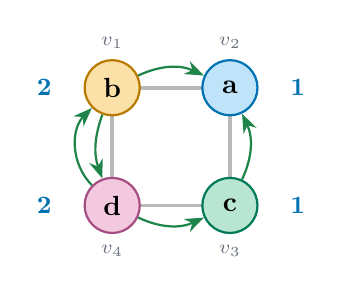
\begin{tikzpicture}[scale=1.15]
  \sqseat{b}{a}{c}{d}{b}{b}
  \draw[like] (b) to[bend left=25] (a);
  \draw[like] (c) to[bend right=25] (a);
  \draw[like] (d) to[bend right=25] (c);
  \draw[like] (b) to[bend right=20] (d);
  \draw[like] (d) to[bend left=45] (b);
  \node[lab] at (0,1.8) {$v_1$}; \node[lab] at (1.3,1.8) {$v_2$};
  \node[lab] at (1.3,-0.5) {$v_3$}; \node[lab] at (0,-0.5) {$v_4$};
  \node[font=\small\bfseries,text=Adraw] at (-0.75,1.3) {2}; \node[font=\small\bfseries,text=Adraw] at (2.05,1.3) {1};
  \node[font=\small\bfseries,text=Adraw] at (2.05,0) {1}; \node[font=\small\bfseries,text=Adraw] at (-0.75,0) {2};
\end{tikzpicture}
\caption{Case 1 on the running example with $s=b$, $w=a$, $t=c$; only $d$ approves $c$, so $d$ takes $v_4$. Green arrows are approvals between neighbours. Every agent attains its maximum possible utility.}
\label{fig:case1}
\end{figure}

\subsection{Case 2: path partitions}

\begin{definition}
A \emph{path partition} of $\cP$ is a collection of directed paths $P_1,\dots,P_k$ covering every agent exactly once. It is \emph{minimal} if $\mathrm{tail}(P_i)\nlikes\mathrm{head}(P_j)$ for all $i\neq j$. The assignment $\Phi(P_1,\dots,P_k)$ seats the paths consecutively around the cycle (Figure~\ref{fig:phi}).
\end{definition}

Inside a path every agent approves its right neighbour, so only path boundaries can contain agents that do not. Let $R(\pi)$ be the number of agents that approve their right neighbour; for a minimal partition with $k\ge2$ paths, $R=n-k$. The initial minimal partition is obtained by repeatedly removing a maximal path: if a tail approved another path's head, one of the two paths could have been extended when it was built.

\begin{figure}[h]
\centering
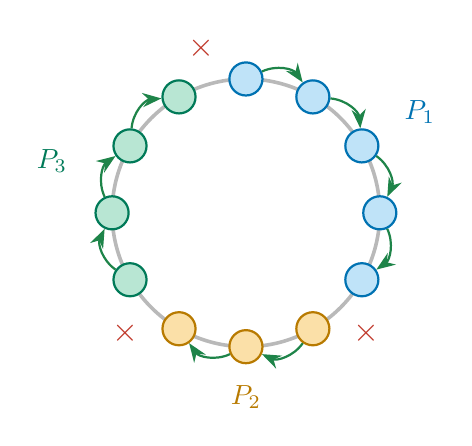
\begin{tikzpicture}[scale=0.85]
  \draw[sedge] (0,0) circle (2);
  \foreach \k/\st in {0/aga,1/aga,2/aga,3/aga,4/aga,5/agb,6/agb,7/agb,8/agc,9/agc,10/agc,11/agc}{
    \node[\st,minimum size=4.2mm] (s\k) at ({90-30*\k}:2) {};}
  \foreach \k in {0,1,2,3,5,6,8,9,10}{\pgfmathtruncatemacro\nx{\k+1}\draw[like] (s\k) to[bend left=40] (s\nx);}
  \foreach \k in {4,7,11}{\node[text=warn,font=\large\bfseries] at ({90-30*(\k+0.5)}:2.55) {$\times$};}
  \node[font=\bfseries,text=Adraw] at (30:3.0) {$P_1$};
  \node[font=\bfseries,text=Bdraw] at (-90:2.75) {$P_2$};
  \node[font=\bfseries,text=Cdraw] at (165:3.0) {$P_3$};
\end{tikzpicture}
\caption{$\Phi(P_1,P_2,P_3)$: paths laid around the cycle (cf.\ paper's Fig.~4). Green: approval of the right neighbour; red crosses: path boundaries.}
\label{fig:phi}
\end{figure}

\begin{claim}[insertion]\label{cl:insert}
In Case 2, if $s\notin P=s_1\to\dots\to s_r$ and $s\to s_r$, then $s\to s_1$ or $s_j\to s\to s_{j+1}$ for some $j$.
\end{claim}
\noindent\emph{Idea.} $s$ and $s_{r-1}$ both approve $s_r$, so (no V) one approves the other. If $s_{r-1}\to s$, insert $s$ between $s_{r-1}$ and $s_r$; otherwise $s\to s_{r-1}$ and we repeat one step back. Formally this is an induction on $r$. This is the only place where the Case 2 assumption is used.

\begin{lemma}\label{lem:repair}
Let $\pi=\Phi(P_1,\dots,P_k)$ for a minimal path partition. If $\pi$ has an adjacent blocking pair, there is a minimal path partition whose assignment $\rho$ satisfies $R(\rho)\ge R(\pi)+1$.
\end{lemma}

Let the blocking pair be $x,y$ at $v_i,v_{i+1}$, with $p$ at $v_{i-1}$ and $z$ at $v_{i+2}$. There are two types.

\paragraph{Type I: $x,y$ consecutive in the same path $P_r$.} The swap rule requires $y\nlikes z$; inside a path $y$ approves its successor, so $y=\mathrm{tail}(P_r)$ and $z=\mathrm{head}(P_{r+1})$. The rule also gives $y\to p$ and $x\to z$. If $|P_r|\ge3$: remove $x,y$ from $P_r$; the rest ends at $p$, and since $y\to p$, Claim~\ref{cl:insert} re-inserts $y$ without changing the tail $p$. Then $p\to x\to z$ glues the result onto $P_{r+1}$ (Figure~\ref{fig:repair}). If $|P_r|=2$: insert $y$ into $P_{r-1}$ (as $y\to p=\mathrm{tail}(P_{r-1})$) and prepend $x$ to $P_{r+1}$. Either way the number of paths drops; gluing further where possible restores minimality, and $R$ increases.

\begin{figure}[h]
\centering
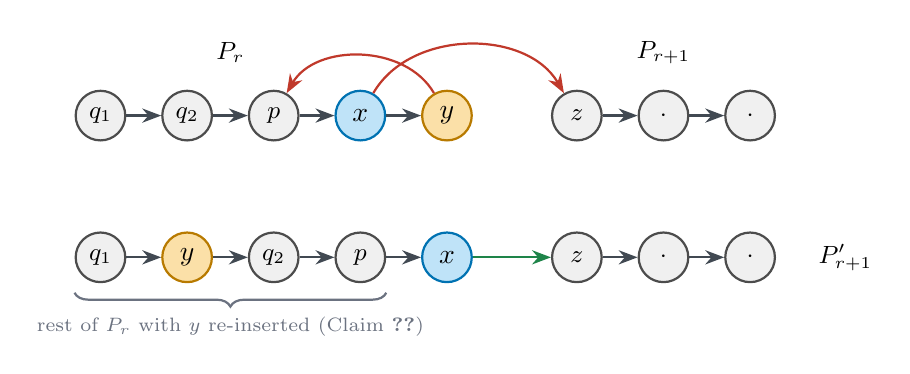
\begin{tikzpicture}[x=1.1cm]
  \node[agg,minimum size=6.3mm] (q1) at (0,1.8) {$q_1$}; \node[agg,minimum size=6.3mm] (q2) at (1,1.8) {$q_2$};
  \node[agg,minimum size=6.3mm] (p) at (2,1.8) {$p$}; \node[aga,minimum size=6.3mm] (x) at (3,1.8) {$x$};
  \node[agb,minimum size=6.3mm] (y) at (4,1.8) {$y$}; \node[agg,minimum size=6.3mm] (z) at (5.5,1.8) {$z$};
  \node[agg,minimum size=6.3mm] (z2) at (6.5,1.8) {$\cdot$}; \node[agg,minimum size=6.3mm] (z3) at (7.5,1.8) {$\cdot$};
  \draw[arc] (q1)--(q2); \draw[arc] (q2)--(p); \draw[arc] (p)--(x); \draw[arc] (x)--(y);
  \draw[arc] (z)--(z2); \draw[arc] (z2)--(z3);
  \draw[bad] (y) to[out=120,in=60] (p); \draw[bad] (x) to[out=60,in=120] (z);
  \node[font=\small\bfseries] at (1.5,2.6) {$P_r$}; \node[font=\small\bfseries] at (6.5,2.6) {$P_{r+1}$};
  \node[agg,minimum size=6.3mm] (b1) at (0,0) {$q_1$}; \node[agb,minimum size=6.3mm] (b2) at (1,0) {$y$};
  \node[agg,minimum size=6.3mm] (b3) at (2,0) {$q_2$}; \node[agg,minimum size=6.3mm] (b4) at (3,0) {$p$};
  \node[aga,minimum size=6.3mm] (b5) at (4,0) {$x$}; \node[agg,minimum size=6.3mm] (b6) at (5.5,0) {$z$};
  \node[agg,minimum size=6.3mm] (b7) at (6.5,0) {$\cdot$}; \node[agg,minimum size=6.3mm] (b8) at (7.5,0) {$\cdot$};
  \draw[arc] (b1)--(b2); \draw[arc] (b2)--(b3); \draw[arc] (b3)--(b4); \draw[arc] (b4)--(b5);
  \draw[like] (b5)--(b6); \draw[arc] (b6)--(b7); \draw[arc] (b7)--(b8);
  \draw[decorate,decoration={brace,mirror,amplitude=5pt},thick,muted] (-0.3,-0.45)--(3.3,-0.45) node[midway,below=5pt,font=\scriptsize] {rest of $P_r$ with $y$ re-inserted (Claim~\ref{cl:insert})};
  \node[font=\small\bfseries] at (8.6,0) {$P'_{r+1}$};
\end{tikzpicture}
\caption{Type I repair with $|P_r|\ge3$ (cf.\ paper's Fig.~5). Red arcs are forced by the blocking pair.}
\label{fig:repair}
\end{figure}

\paragraph{Type II: $x=\mathrm{tail}(P_r)$, $y=\mathrm{head}(P_{r+1})$.} The swap rule requires $y\nlikes z$. If $|P_{r+1}|\ge2$, then $y$ approves its successor $z$; so $P_{r+1}=\{y\}$ and $z=\mathrm{head}(P_{r+2})$. The rule also requires $x\to z$, i.e.\ $\mathrm{tail}(P_r)\to\mathrm{head}(P_{r+2})$, which contradicts minimality. So Type II cannot occur. (See Section~\ref{sec:gaps} for two boundary cases.)

\paragraph{Termination and running time.} $R\le n$ and each application of Lemma~\ref{lem:repair} increases $R$, so at most $n$ repairs occur, and the final assignment has no adjacent blocking pair. The paper states that each repair takes $O(n^2)$ time. Our reconstruction: finding an adjacent blocking pair is $O(n)$ (four look-ups per pair by the swap rule); the insertion of Claim~\ref{cl:insert} walks back along one path in $O(n)$; gluing lists is $O(n)$; restoring minimality checks tail--head pairs, at most $O(k^2)=O(n^2)$, and each glue only creates one new tail and head to recheck. Overall:
\begin{center}
\begin{tabular}{@{}ll@{}}
\toprule
Step & Cost \\
\midrule
Decide the case (all triples) & $O(n^3)$ \\
Case 1 greedy & $O(n^2)$ \\
Case 2: initial minimal partition & $O(n^2)$ \\
Case 2: at most $n$ repairs of $O(n^2)$ each & $O(n^3)$ \\
\bottomrule
\end{tabular}
\end{center}
\textbf{[Ours]} The case check as described (examining triples) needs $\Theta(n^3)$ time in the worst case: when no V exists it must examine every pair of in-neighbours of every agent, and for a transitive tournament this is about $n^3/6$ pairs. Whether a faster algorithm exists is not addressed in the paper.

\paragraph{Back to Proposition~\ref{prop:loop}.} The looping instance is in Case 2. If the algorithm's first maximal path is $c\to a\to b\to d$ (which covers every agent, and $d\to c$), then wrapped around the cycle every agent approves its right neighbour ($R=4$) and the assignment is NS at once, although swap dynamics from $\pi$ never reaches an NS assignment. A different choice of maximal paths can start from the partition $\{a\to d\to c,\ b\}$ instead; this case is discussed in Section~\ref{sec:gaps}.

\paragraph{Course connection.} $R$ is a progress measure in the spirit of the energy of Hopfield networks. Unlike the potentials behind PLS (Polynomial Local Search) problems, it takes at most $n+1$ values, so the number of improving steps is polynomial. Note that the steps are re-arrangements made by the algorithm, not swaps made by agents.

\subsection{Why distance-2 stability fails on cycles [ours]}\label{sec:c5}

On paths the paper obtains the stronger guarantee of no blocking pair within distance $2$ (Theorem~\ref{thm:path}); on cycles this is impossible by the five-agent instance of Berriaud et al. The paper does not reproduce their instance; we found the following one by computer search. On $C_5$ every two seats are at distance $1$ or $2$, so distance-2 stability coincides with stability. Let
\[
a\to c,e;\quad b\to a,e;\quad c\to a,d;\quad d\to b,c;\quad e\to b,d,
\]
i.e.\ mutual pairs $a\leftrightarrow c$, $c\leftrightarrow d$, $b\leftrightarrow e$ and the directed $4$-cycle $a\to e\to d\to b\to a$. Up to rotation and reflection there are $12$ seatings, and each has a blocking pair:
\begin{center}
\small
\begin{tabular}{@{}lcclc@{}}
\toprule
Seating & Pair & Distance & Gains & NS? \\
\midrule
$a\,b\,c\,d\,e$ & $c,e$ & 2 & $1\to2$, $1\to2$ & yes \\
$a\,b\,c\,e\,d$ & $a,c$ & 2 & $0\to1$, $0\to1$ & no \\
$a\,b\,d\,c\,e$ & $a,e$ & 1 & $1\to2$, $0\to1$ & no \\
$a\,b\,d\,e\,c$ & $b,c$ & 2 & $1\to2$, $1\to2$ & yes \\
$a\,b\,e\,c\,d$ & $a,e$ & 2 & $0\to1$, $1\to2$ & yes \\
$a\,b\,e\,d\,c$ & $a,d$ & 2 & $1\to2$, $1\to2$ & yes \\
$a\,c\,b\,d\,e$ & $b,d$ & 1 & $0\to1$, $1\to2$ & no \\
$a\,c\,b\,e\,d$ & $b,d$ & 2 & $1\to2$, $0\to1$ & yes \\
$a\,c\,d\,b\,e$ & $b,e$ & 1 & $1\to2$, $1\to2$ & no \\
$a\,c\,e\,b\,d$ & $a,c$ & 1 & $1\to2$, $1\to2$ & no \\
$a\,d\,b\,c\,e$ & $a,e$ & 1 & $1\to2$, $0\to1$ & no \\
$a\,d\,c\,b\,e$ & $c,d$ & 1 & $1\to2$, $1\to2$ & no \\
\bottomrule
\end{tabular}
\end{center}
Five of the seatings are NS, as Theorem~\ref{thm:cycle} requires; their only blocking pairs are at distance $2$.

The path proof does not transfer because it uses two features a cycle lacks: the first seat is an endpoint (anyone swapping into it loses a neighbour), and the greedy guarantee runs in one direction only, so on a cycle the pairs around the point where the last seat meets the first are unconstrained. Case 1 above seats a V first precisely to make that junction safe for adjacent swaps; distance $2$ would require control two seats away on both sides.

% =====================================================================
\section{Path seat graphs}

\begin{theorem}\label{thm:path}
If the seat graph is a path, an assignment with no blocking pair within distance $2$ exists and can be computed in $O(n^2)$ time. (The paper states $O(n^3)$; the bound $O(n^2)$ is our analysis of the same algorithm.)
\end{theorem}

\paragraph{Algorithm.} Seat any agent on $v_1$. For $k=2,\dots,n$, seat on $v_k$ an unseated agent who approves the agent on $v_{k-1}$ if one exists, and otherwise any unseated agent. Each of the $n$ steps scans at most $n$ unseated agents with one look-up each, giving $O(n^2)$.

\paragraph{Correctness.} The agents on $v_2$ and $v_3$ never envy the agent on $v_1$: after such a swap their neighbourhood is a subset of their current one. For $i\ge2$, let $x$ be the agent on $v_i$.
\begin{itemize}
  \item If $x$ approves its left neighbour, then after a swap with $v_{i+1}$ or $v_{i+2}$ it can gain only by reaching utility $2$, which requires approving the agent on $v_{i+1}$ (a neighbour in both swapped positions); but then $x$ already has utility $2$.
  \item If $x$ does not approve its left neighbour, then by construction neither the agent on $v_{i+1}$ nor the one on $v_{i+2}$ approves it (otherwise it would have been chosen instead of $x$). After swapping with $x$, the only new neighbour of either agent is that left neighbour, so neither gains.
\end{itemize}

\paragraph{Running example.} Starting from $a$: $c\to a$, then $d\to c$, then $b\to d$, giving $(a,c,d,b)$ (Figure~\ref{fig:path}), which is in fact stable.

\begin{figure}[h]
\centering
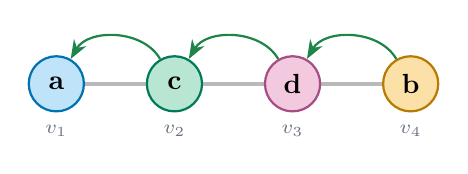
\begin{tikzpicture}
  \pathseat{a}{c}{d}{b}
  \draw[like] (c) to[out=120,in=60] (a);
  \draw[like] (d) to[out=120,in=60] (c);
  \draw[like] (b) to[out=120,in=60] (d);
  \seatlabels
\end{tikzpicture}
\caption{Theorem~\ref{thm:path} on the running example: each new agent approves the previous one.}
\label{fig:path}
\end{figure}

\paragraph{Context and course connection.} Berriaud et al.\ showed by a potential argument that swap dynamics on paths converge to an assignment with no blocking pair within distance $2$, gave evidence that convergence may take exponentially many steps, and left open whether such an assignment can be computed in polynomial time. This is the PLS phenomenon from the course: improvement must stop, but possibly only after exponentially many steps. The paper settles the question by a direct construction that does not simulate the dynamics.

% =====================================================================
\section{A sufficient condition for general seat graphs}

\begin{definition}
A set $X\subseteq A$ is a \emph{directed feedback vertex set} (DFVS) if $\cP[A\setminus X]$ is acyclic; the DFVS number $\gamma$ is the minimum size of such a set. A \emph{leaf} of $G$ is a vertex of degree one.
\end{definition}

\begin{theorem}\label{thm:dfvs}
If the number of leaves of $G$ exceeds the DFVS number $\gamma$ of $\cP$, there exists an NS assignment on $G$. When $\gamma=0$, i.e.\ $\cP$ is a DAG, a stable assignment can be computed in polynomial time.
\end{theorem}

The proof only uses that a DFVS fits on the leaves, i.e.\ $\gamma\le\#$leaves (Section~\ref{sec:gaps}).

\paragraph{Sinks.} A \emph{sink} of a directed graph is a vertex with no outgoing arcs. Every DAG has one: following arcs from any vertex can never revisit a vertex, so the walk ends at a vertex with no outgoing arc. Removing a sink leaves a DAG, so the agents of $A\setminus X$ can be ordered $s_1,s_2,\dots$ with $s_\ell$ a sink of $\cP[A\setminus(X\cup\{s_1,\dots,s_{\ell-1}\})]$. Consequently everyone approved by $s_i$ lies in $X\cup\{s_1,\dots,s_{i-1}\}$.

\paragraph{Algorithm.}
\begin{enumerate}
  \item Seat the agents of a smallest DFVS $X$ on leaves.
  \item In the order $s_1,s_2,\dots$, let each agent take the free seat with the largest number of already-seated approved neighbours (ties broken arbitrarily).
\end{enumerate}

\paragraph{Correctness.} Take $i<j$. When $s_i$ chose, all agents it approves were seated and never move afterwards, and the seat of $s_j$ was still free. So $s_i$ judged that seat at most as good, and after a swap its approved neighbours there are the same (it does not approve $s_j$). Hence $s_i$ never envies a later agent, and no blocking pair (at any distance) consists of two agents outside $X$. Now let $x\in X$ sit on a leaf with unique neighbour $y$. If $y$ swaps onto the leaf, its only neighbour becomes $x$, whom it already had, so $y$ does not envy $x$. Hence there is no adjacent blocking pair. If $X=\emptyset$ there is no blocking pair at all.

\paragraph{The seat choice matters [ours].} On the running example with seats $v_1v_2v_3v_4$ (a path), the two 2-cycles $a\leftrightarrow c$, $b\leftrightarrow d$ are disjoint, so $\gamma=2$; take $X=\{a,b\}$ on the leaves $v_1,v_4$. Among $c,d$ we have $d\to c$, so $c$ is the sink and chooses first; it approves $a$, so it takes $v_2$, and $d$ takes $v_3$. The result $(a,c,d,b)$ is NS (indeed stable). Had $c$ taken $v_3$ instead, the result $(a,d,c,b)$ gives $u_c=0$ and $u_d=1$, and swapping $c,d$ raises them to $1$ and $2$: an adjacent blocking pair. Note also that this example has $\gamma=2=\#$leaves, which the proof covers but the literal statement (``exceeds'') does not.

\paragraph{Consequence.} Planar directed graphs have DFVS number at most $\tfrac35n$ (via Borodin's acyclic colouring theorem), so for planar preference graphs an NS assignment exists on every seat graph with at least $60\%$ leaves, for example full $m$-ary trees with $m\ge3$, which have at least $\frac{m-1}{m}n$ leaves.

\paragraph{Course connection [ours].} The argument mirrors the existence argument for colouring games on DAGs: agents choose in reverse topological order, sinks first, so no later choice can undermine an earlier one. Here the DAG is the \emph{preference} graph; in Theorem~\ref{thm:cycle} the cycle is the \emph{seat} graph.

% =====================================================================
\section{Critical remarks [ours]}\label{sec:gaps}

\subsection{Two cases missing from the proof of Lemma~\ref{lem:repair}}

The Type II argument derives $\mathrm{tail}(P_r)\to\mathrm{head}(P_{r+2})$ and appeals to minimality, which only forbids $\mathrm{tail}(P_i)\to\mathrm{head}(P_j)$ for $i\ne j$. The Type I argument glues the repaired path onto $P_{r+1}$ and counts on the number of paths dropping. Both steps break when there are very few paths (indices are taken modulo $k$).

\paragraph{Gap 1: Type II with $k=2$.} Then $P_{r+2}=P_r$, and $x\to z$ says that $P_r$'s tail approves its own head, which minimality allows. \emph{Example:} in the instance of Proposition~\ref{prop:loop}, the partition $\{a\to d\to c,\ b\}$ is minimal ($c\nlikes b$ and $b\nlikes a$), and $\Phi$ seats $a,d,c,b$ around the cycle. With $(x,y,p,z)=(c,b,d,a)$ we have $c\to a$, $c\nlikes d$, $b\to d$, $b\nlikes a$: a Type II blocking pair.

\emph{Patch.} In this case $P_r$ closes into a directed cycle (its tail approves its head) and $y\to p$ with $p\in P_r$ the predecessor of $x$. Cut the cycle just before $p$ and prepend $y$: $y\to p\to x\to z\to\cdots$ is a single path covering all agents, so $k$ drops from $2$ to $1$ and $R$ increases. In the example this gives $b\to d\to c\to a$.

\paragraph{Gap 2: Type I with $k=1$.} Then $P_{r+1}=P_r$, so ``glue onto $P_{r+1}$'' is not available and the number of paths cannot drop below one. \emph{Example:} $a\to b$, $a\to c$, $b\to c$, $b\to d$, $c\to d$, $d\to a$ (Case 2). The maximal path $b\to d\to a\to c$ seated around the cycle has the Type I blocking pair $x=a$, $y=c$ (with $p=d$, $z=b$).

\emph{Patch.} Remove $x,y$; re-insert $y$ by Claim~\ref{cl:insert}. Since $y\nlikes z$, $y$ is not prepended, so the path still starts at $z$ and ends at $p$. Appending $x$ gives a path ending in $x$ with $x\to z$, a Hamiltonian cycle of $\cP$: $R$ rises from $n-1$ to $n$, and an assignment in which every agent approves its right neighbour is NS: in any adjacent pair, the right agent approves its own right neighbour, so by the swap rule it does not envy the left agent. In the example the result is $b\to c\to d\to a\to b$.

\paragraph{Evidence.} We implemented Algorithm~1 as written in the paper together with both patches and ran it on $60{,}000$ random instances with $4$ to $9$ agents ($17{,}592$ of them in Case 2). Gap 1 occurred $106$ times and Gap 2 $644$ times; the paper's contradiction for Type II with three or more paths was never violated; $R$ increased at every repair; and every output was NS. Independently, every one of the $4096$ preference graphs on four agents admits an NS assignment on $C_4$. We therefore believe Theorem~\ref{thm:cycle} is correct and the gaps are in the write-up only.

\subsection{Theorem~\ref{thm:dfvs}: statement versus proof}
\begin{itemize}
  \item The statement requires the number of leaves to \emph{exceed} $\gamma$, but the proof uses only $|X|\le|L|$, and the introduction says ``upper bounded by''. The running example ($\gamma=2=\#$leaves) is covered by the proof but not by the statement.
  \item The abstract and introduction speak of a polynomial-time algorithm whenever the DFVS is at most the number of leaves, while the theorem claims polynomial time only for $\gamma=0$. For $\gamma>0$ the algorithm needs a small enough DFVS, and finding a minimum DFVS is NP-hard in general (Karp, 1972); the paper does not explain how to find $X$ efficiently.
\end{itemize}

\subsection{Running time of the path algorithm}
As shown in Theorem~\ref{thm:path}, the greedy runs in $O(n^2)$, which is tighter than the stated $O(n^3)$.

\subsection{Who finds the stable seating?}
The motivation is agents arranging swaps with their neighbours, but on cycles such swaps may never reach an NS assignment (Proposition~\ref{prop:loop}). The positive results therefore guarantee what a central planner can compute, not where decentralised behaviour leads. On paths the dynamics do converge (Berriaud et al.), but possibly slowly.

% =====================================================================
\section{Connections to the course}

\begin{center}
\renewcommand{\arraystretch}{1.25}
\begin{tabular}{@{}p{4.6cm}p{10cm}@{}}
\toprule
\textbf{Course topic} & \textbf{Where it appears} \\
\midrule
Hedonic games & Utility is additively separable with 0/1 values, over the seat neighbourhood rather than a coalition. \\
Potential games, FIP, generalised ordinal potentials & Proposition~\ref{prop:loop} is an improvement cycle, so no potential exists for swap dynamics on cycles; with symmetric preferences the number of mutually approving adjacent pairs is a potential. \\
Weakly acyclic games & From the assignment of Proposition~\ref{prop:loop}, every improvement path cycles. \\
Hopfield networks, progress measures & The count $R$ in Lemma~\ref{lem:repair} rises with each repair and takes at most $n+1$ values. \\
PLS & On paths, swap dynamics converge but possibly in exponential time; Theorem~\ref{thm:path} constructs the outcome directly. \\
Colouring games on DAGs & Theorem~\ref{thm:dfvs} lets sinks choose first, as in the existence proof for DAGs. \\
\bottomrule
\end{tabular}
\end{center}

% =====================================================================
\section{Open questions and conclusion}

The paper lists the following directions: other seat graphs such as grids and trees, and more conditions in the style of Theorem~\ref{thm:dfvs}; efficiency, i.e.\ bounding the price of neighbourhood stability or maximising welfare subject to NS; and preferences beyond binary, where cycles already fail with cardinal values and paths remain open.

To conclude: restricting swaps to neighbours turns a notion that frequently fails into one that is guaranteed on cycles and paths, although it can still fail on dense seat graphs such as $K_{t,t}$. The main technical idea, laying out path partitions of the preference graph around the cycle and repairing blocking pairs by merging paths, gives a polynomial algorithm in a setting where the natural dynamics can cycle forever. Our checks support all the paper's results, and identify two small cases in the main lemma's proof that need the patches above.

% =====================================================================
\appendix
\section{Computational verification}\label{app:verify}

To guard against errors in our own reading, we checked the small examples and our additional claims with short Python programs written for this report. Agents, seat graphs and approvals are stored explicitly; utilities and blocking pairs are computed directly from the definitions in Section~2.

\paragraph{Exhaustive checks.}
\begin{itemize}
  \item Running example: $b,d$ is the only adjacent blocking pair of $(a,d,b,c)$; $(a,b,d,c)$ is stable; the Case 1 output $(b,a,c,d)$ on $C_4$ is NS; $(a,c,d,b)$ on the path is stable; $(a,d,c,b)$ has the adjacent blocking pair $c,d$.
  \item Proposition~\ref{prop:loop}: the four swaps return to $\pi$, the blocking pair is unique at every step, and $8$ of the $24$ seatings are NS.
  \item Theorem~\ref{thm:kTT} for $t=3$: none of the $720$ assignments on $K_{3,3}$ is NS. For $t=4$ the assignment given in the text gives every agent utility $2$.
  \item Example~2: all $720$ assignments are NS and none is stable.
  \item The $\pm1$ example on a path of three seats: no seating is NS.
  \item Theorem~\ref{thm:cycle} for $n=4$: each of the $4096$ preference graphs on four agents has an NS assignment on $C_4$.
  \item The five-agent instance of Section~\ref{sec:c5}: no stable seating on $C_5$; $10$ of the $24$ seatings with $a$ fixed on one seat are NS (5 up to reflection).
  \item The two examples of Section~\ref{sec:gaps}: each has the stated blocking pair, and the patched assignment is NS.
\end{itemize}

\paragraph{Randomised checks.}
\begin{itemize}
  \item Theorem~\ref{thm:path}: $20{,}000$ random instances with $3$ to $8$ agents; the greedy output never had a blocking pair within distance $2$.
  \item Theorem~\ref{thm:cycle}: Algorithm~1 implemented as in the paper, with the two patches of Section~\ref{sec:gaps}, on $60{,}000$ random instances with $4$ to $9$ agents. At every repair the program asserted the properties used in the proof (the type of the blocking pair, the arcs forced by the swap rule, the success of Claim~\ref{cl:insert}, and the increase of $R$); all outputs were NS.
\end{itemize}

These checks support the statements but are not proofs; for larger instances we rely on the arguments given in the text.

% =====================================================================
\begin{thebibliography}{9}\small
\bibitem{main} H.~Aziz, G.~Lisowski, M.~Suzuki and J.~Vollen. Neighborhood stability in assignments on graphs. arXiv:2407.05240, 2024.
\bibitem{berriaud} D.~Berriaud, A.~Constantinescu and R.~Wattenhofer. Stable dinner party seating arrangements. WINE 2023; arXiv:2305.09549.
\bibitem{bodlaender} H.~L.~Bodlaender, T.~Hanaka, L.~Jaffke, H.~Ono, Y.~Otachi and T.~C.~van der Zanden. Hedonic seat arrangement problems. AAMAS 2020.
\bibitem{bilo} D.~Bil\`o, V.~Bil\`o, P.~Lenzner and L.~Molitor. Topological influence and locality in swap Schelling games. Autonomous Agents and Multi-Agent Systems 36(2), 2022.
\bibitem{bullinger} M.~Bullinger and W.~Suksompong. Topological distance games. Theoretical Computer Science 981, 2024.
\bibitem{massand} S.~Massand and S.~Simon. Graphical one-sided markets. IJCAI 2019.
\bibitem{borodin} O.~V.~Borodin. On acyclic colorings of planar graphs. Discrete Mathematics 25(3), 1979.
\bibitem{monderer} D.~Monderer and L.~S.~Shapley. Potential games. Games and Economic Behavior 14(1), 1996.
\bibitem{karp} R.~M.~Karp. Reducibility among combinatorial problems. In Complexity of Computer Computations, 1972.
\end{thebibliography}

\end{document}
